%!TEX root = ../main.tex

\chapter{HARQ}
\label{chp:analysis}

\section{Concurrent processes limit}

One of the problems highlighted by the \ac{3GPP} technical report \cite{3gpp-tr-38.811} on the matter of non-terrestrial networks regards the maximum number of concurrent \ac{HARQ} processes. 

\subsection{Problem description}
The details of \ac{HARQ} protocol implementation in the 5G \ac{NR} standard is extensively treated in many publications such as \cite{harq-wireless-communications-survey}. However, for the purpose of understanding what is a \ac{HARQ} process and how it affects the throughput in a non-terrestrial scenario, a brief overview of a few key concepts is enough.

\begin{figure}[ht]
    \centering
    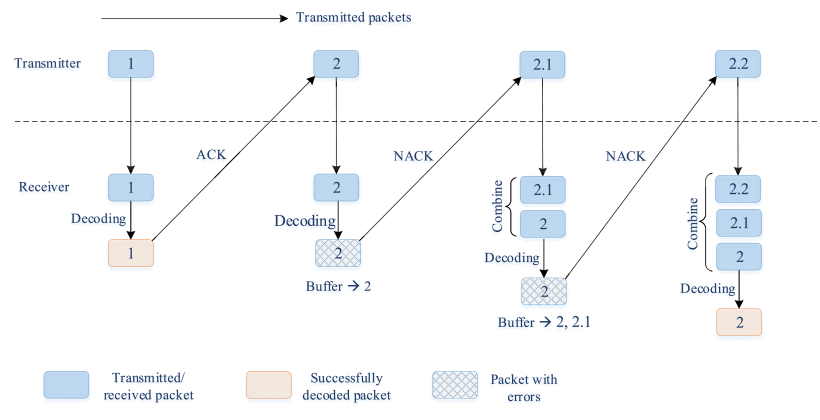
\includegraphics[width=0.9\textwidth]{res/harq-retx-scheme.png}
    \caption{\ac{HARQ} retransmission diagram \cite{harq-wireless-communications-survey}}
    \label{fig:harq_retx_scheme}
\end{figure}

\subsubsection{HARQ working principle}
\paragraph{}
Fig. \ref{fig:harq_retx_scheme} gives an overview of how \ac{HARQ} processes work. Upon successful reception, depicted in the first column of Fig. \ref{fig:harq_retx_scheme}, an \ac{ACK} is sent back, triggering the transmission of the successive \ac{TB}, which is represented in the second column. This behavior is the normal state in which transmissions are received correctly, and it keeps repeating itself until errors are detected.

\paragraph{} Should the receiver detect errors in the received \ac{TB}, represented by the greyed packet, a \ac{NACK} is relayed back to the sender, which in turn proceeds to send some additional redundancy bits. Note that the sender does not repeat the whole \ac{TB}. The receiver now proceeds to decode the transfer block using all the information that it has received so far.

This is the most important feature of \ac{HARQ} protocol: it does not discard the packets affected by errors, since they can be at least used to recover some information. The erroneous packets are stored in buffers and used for joint decoding \cite{5g-nr-harq-devopedia}. 

\paragraph{} If the redundancy bits that the sender just transmitted are still not enough to allow for a correct decoding of the transfer block, or if another error is detected, a retransmission is triggered. This is shown in the last column of Fig. \ref{fig:harq_retx_scheme}, where all the packets received so far contribute in correctly decoding packet 2.

Finally, if even this retransmission is affected by errors and the combination of the information received so far is not enough to complete the decoding of the \ac{TB}, additional information is sent. After this fourth interaction, no further attempts are made to correct the packet \cite{5g-nr-harq-sharetechnote}.

\paragraph{} The various transmissions and retransmissions being made by the protocol are called \ac{RV} 


\subsubsection{Stop and wait}
\paragraph{} The presented behavior means that \ac{HARQ} is a stop-and-wait kind of protocol, since it is designed to wait for the arrival of previous packet's \ac{ACK} before sending the new one. While this enforces the delivery of ordered packets, it also brings the downside of severely underutilizing the channel capacity, wasting resources that could potentially be used for transmission instead \cite{3gpp-ts-38.214}.

This limitation is overcome by the introduction of multiple concurrent processes.

\subsubsection{Processes}
\paragraph{}
A \ac{HARQ} process starts when a \ac{TB} is passed to the \ac{HARQ} entity and finishes when the \ac{ACK} relative to that same \ac{TB} is received by the sender. After the \ac{ACK} is correctly received, the next \ac{TB} starts being processed. Considering a link with propagation delay $\tau_p$, the minimum active time for a process is therefore $2\tau_p$, i.e. the time for the transfer block to arrive to the destination plus the time for the acknowledgement to travel back to the sender.

The 5G \ac{NR} standard allows the base station to configure the maximum number of concurrent \ac{HARQ} processes to be assigned to each connected user, with the default value being of 8 concurrent processes and the maximum 16 \cite{3gpp-ts-38.300, 5g-nr-harq-devopedia}. 

\subsubsection{Application in NTNs}
\paragraph{}
Since the propagation delay of \ac{NTNs} is order of magnitude larger than their terrestrial counterpart, the limited maximum number of concurrent processes lowers the maximum achievable throughput, as detailed in the following toy example. 

\paragraph{Example} Consider a scenario where each process tries to send a \ac{TB} every $2\tau_p$, which is the maximum rate at which transfer blocks can be sent under the condition of waiting for the acknowledgement to arrive before starting a new transmission, to a \ac{LEO} satellite orbiting at 2.000Km, therefore having $\tau_p\approx6$ms. Assuming the best possible conditions with no need for retransmissions and assuming that the base station grants the \ac{UE} to the best possible clearance of 16 concurrent processes, the total send rate is of 16 transfer blocks every 12ms. In order to target a throughput of 50Mbps, the block size must therefore be of at least $$\frac{\textit{target throughput} \times 2\tau_p}{\textit{number of processes}} = 37,5Kb$$
Doing the same calculation for a terrestrial scenario with the \ac{gNB} placed at a distance of 600m from the \ac{UE}, we obtain that the minimum \ac{TBS} must be of just $12b$.
Both calculations do not factor in overheads, control information, channel access requests and processing delays, but are helpful to give an idea of the disproportion between the two conditions.

While the necessary block size for the \ac{NTN} case is technically possible to achieve even with 4G, it necessitates a high \ac{SNR} to work properly. This constraint becomes even more conservative in the non-terrestrial case, since retransmissions adds delays in multiples of propagation delay and are therefore more costly \cite{4g-phy-processing-sharetechnote}.

\subsection{Possible solutions}
\paragraph{Increasing the processes}
The easiest solution would be to increase the number of maximum concurrent \ac{HARQ} processes. However, this comes with some caveats mainly regarding the higher computational capabilities required and higher power consumption, that can quickly become problematic in battery-operated equipments such as smartphones. Each process also requires the presence of a buffer on both the receiver side and the sender side, so additional resources are required at the \ac{gNB}, too. 
\paragraph{Aggressive HARQ}
A more sophisticated approach could involve the design of an aggressive version of the \ac{HARQ} protocol, where each process is allowed to send multiple packets before receiving an acknowledgement. Since there already are multiple concurrent processes, each \ac{ACK} packet must already contain a field specifying the number of process it belongs to, and the information identifying the specific packet to be acknowledged within a process could be encoded inside this field.
\paragraph{Disable \ac{HARQ}}
Lastly, the option of disabling \ac{HARQ} completely and rely solely on \ac{ARQ} retransmissions has been proposed by 3GPP itself\cite{hybrid-arq-schemes-muk}. This, however, would come with a performance penalty since satellite links typically suffer from more severe conditions than terrestrial ones, and \cite{5g-beyond-5g-ntn-trends-vanellicoralli} demonstrated that a version of \ac{HARQ} specifically designed for non-terrestrial networks would be beneficial.


\subsection{Simulator configuration}
While the number of concurrent HARQ processes can be configured in ns-3, it cannot exceed the value of 100. By performing some simple calculations, knowing that the \ac{SNR} conditions allow for the transmissions of \ac{TB}s with size of 1024B, to achieve a target throughput of 50Mbps on the best case of 6ms $\tau_p$ the necessary processes would be 74.
$$\frac{\textit{target throughput} \times 2\tau_p}{\textit{total block size}} \approx 74 \textit{processes}$$

This does not account for the delays caused by retransmissions, so simulator crashes due to processes overflow are frequent while testing even the best case scenario.

